\newpage
\section*{Tables and Figures}

% Table 1: Parameter Values
\begin{table}[h!]
    \centering
    \begin{tabular}{|c|c|c|c|}
    \hline
    \textbf{Variable} & \textbf{Description}                                                 & \textbf{Value} & \textbf{Unit} \\ \hline
    g      & Gravitational Acceleration & 9.81 & $\dfrac{m}{s^2}$ \\ \hline
    m      & Quadcopter Mass & 0.468 & kg            \\ \hline
    l      & Quadcopter Arm Length & 0.225          & m             \\ \hline
    k      & Propeller Lift Coefficient &       $2.980 \cdot 10^{-6}$        & --            \\ \hline
    b      & Propeller Drag Coefficient &       $1.140 \cdot 10^{-7}$         & --            \\ \hline
    $I_{xx}$ & Inertia Matrix R1C1        &         $4.856 \cdot 10^{-3}$       &  $kg \cdot m^2$             \\ \hline
    $I_{yy}$ & Inertia Matrix R2C2        &     $4.856 \cdot 10^{-3}$           &    $kg \cdot m^2$           \\ \hline
    $I_{zz}$ & Inertia Matrix R3C3        &     $8.801 \cdot 10^{-3}$           &    $kg \cdot m^2$           \\ \hline
    U        & Inertial Frame Force x Component & Variable & N  \\ \hline
    V        & Inertial Frame Force y Component & Variable & N  \\ \hline
    W        & Inertial Frame Force z Component & Variable & N  \\ \hline
    $\phi$   & Inertial Frame Euler Angle About x Axis & Variable & rad  \\ \hline
    $\theta$ & Inertial Frame Euler Angle About y Axis & Variable & rad  \\ \hline
    $\psi$   & Inertial Frame Euler Angle About z Axis & Variable & rad  \\ \hline
    P        & Inertial Frame Moment About x Axis & Variable & N$\cdot$m  \\ \hline
    Q        & Inertial Frame Moment About y Axis & Variable & N$\cdot$m  \\ \hline
    R        & Inertial Frame Moment About z Axis & Variable & N$\cdot$m  \\ \hline
    h        & Quadcopter Height in Inertial Frame & Variable & m  \\ \hline
    \end{tabular}
    \caption{Variable Descriptions and Values}
\end{table}

% Table 2: PID Controller Parameters
\begin{table}[h!]
    \begin{tabular}{|c|l|l|l|l|}
    \hline
    \textbf{Controller} & \multicolumn{1}{c|}{\textbf{P}} & \multicolumn{1}{c|}{\textbf{I}} & \multicolumn{1}{c|}{\textbf{D}} & \multicolumn{1}{c|}{\textbf{N}}        \\ \hline
    h                   & 0.667090759823057               & 0.0833409544861024              & 1.3246835477396                 & 326.5222788690   \\ \hline
     $\Phi$                   & 0.006797426033441             & 0.0001265287568533            & 0.0097998134935             & 11.93198682033  \\ \hline
         $\Theta$               & 0.006797426033441             & 0.0001265287568533            & 0.0097998134935             & 11.93198682033  \\ \hline
        $\Psi$                & 3.04588477387e-11             & 1.691044011866e-13            & 2.5758358949e-10            & 0.520960333232 \\ \hline
    \end{tabular}
    \caption{PID Controller Parameters for Simulink}
\end{table}


% Quadcopter
\begin{figure}[h]
    \centering
    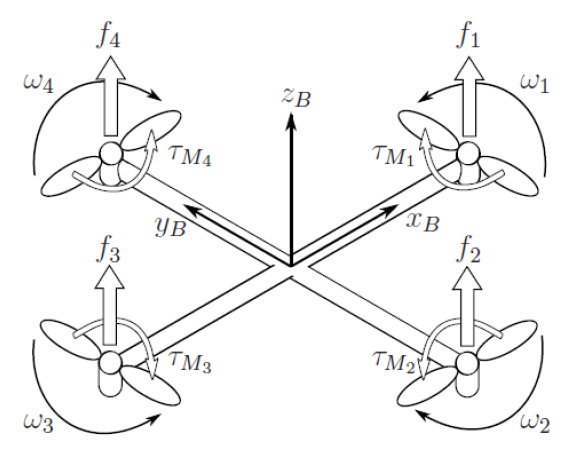
\includegraphics[width=0.7\textwidth]{01_quadcopter}
    \caption{A Quadcopter and Body Frame Axes}
    \label{fig:quad}
\end{figure}

% Force Equations
\begin{figure}[h]
    \centering
    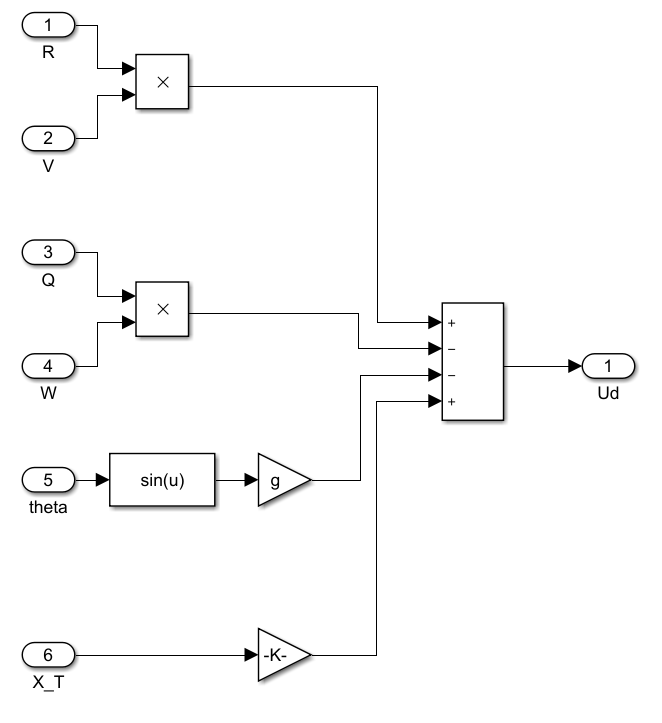
\includegraphics[width=\textwidth]{02_Udot}
    \caption{$\dot{U}$ Equation (2) Simulink Implementation}
    \label{fig:Udot}
\end{figure}

\begin{figure}[h]
    \centering
    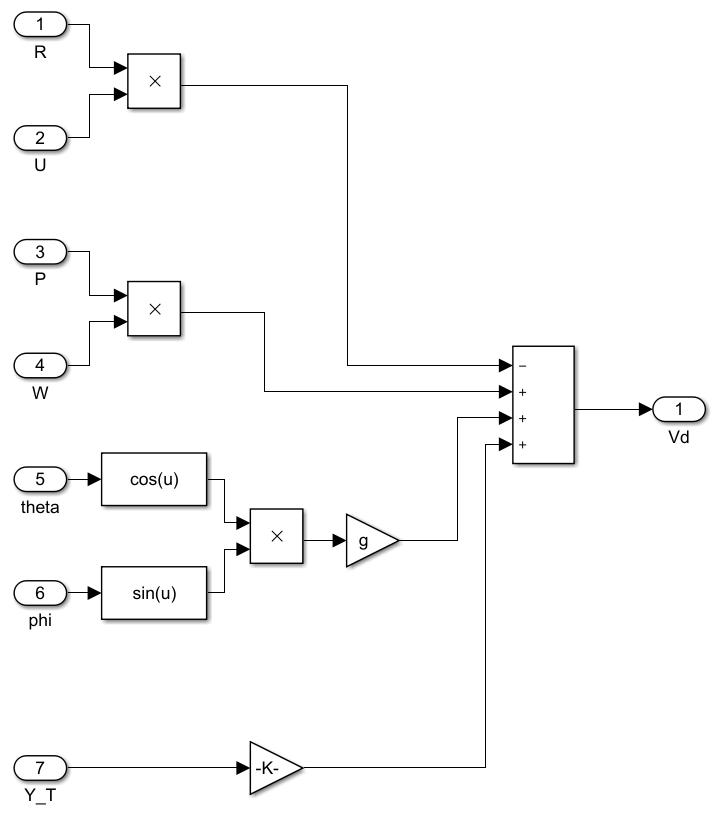
\includegraphics[width=\textwidth]{03_Vdot}
    \caption{$\dot{V}$ Equation (3) Simulink Implementation}
    \label{fig:Vdot}
\end{figure}

\begin{figure}[h]
    \centering
    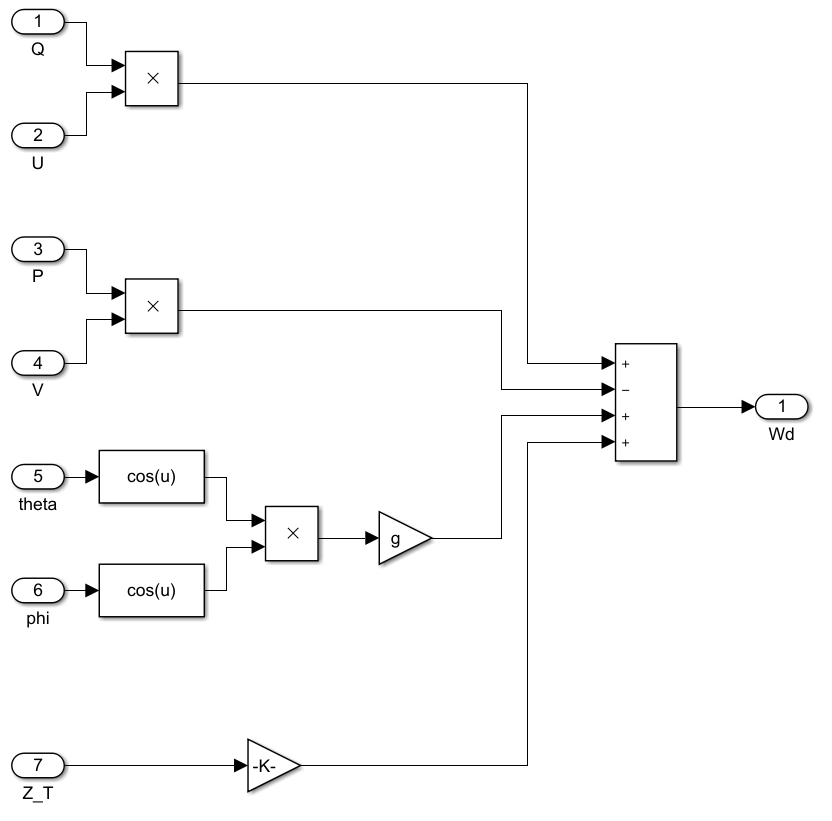
\includegraphics[width=\textwidth]{04_Wdot}
    \caption{$\dot{W}$ Equation (4) Simulink Implementation}
    \label{fig:Wdot}
\end{figure}

\begin{figure}[h]
    \centering
    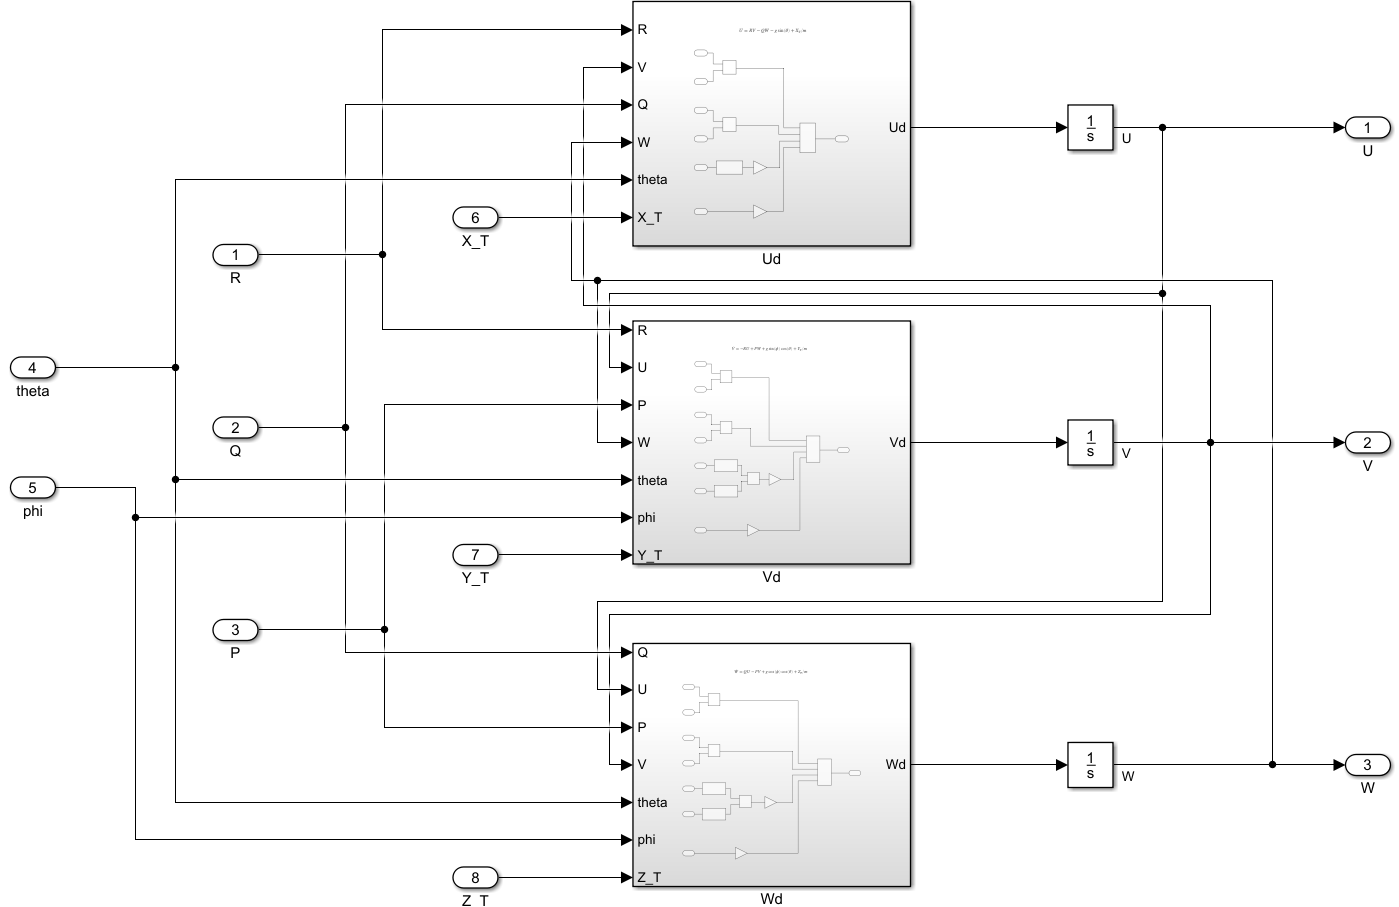
\includegraphics[width=\textwidth]{05_force_equations}
    \caption{All 3 Force Equation Subsystems Connected in Simulink}
    \label{fig:force_eqns}
\end{figure}

% Kinematic Equations
\begin{figure}[h]
    \centering
    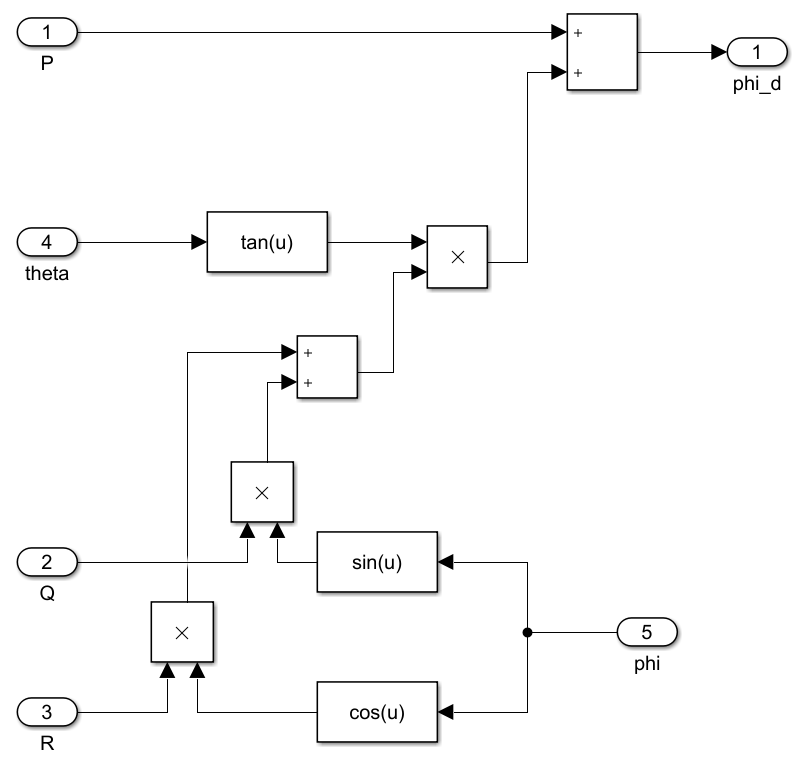
\includegraphics[width=\textwidth]{06_Phid}
    \caption{$\dot{\Phi}$ Equation (5) Simulink Implementation}
    \label{fig:phid}
\end{figure}

\begin{figure}[h]
    \centering
    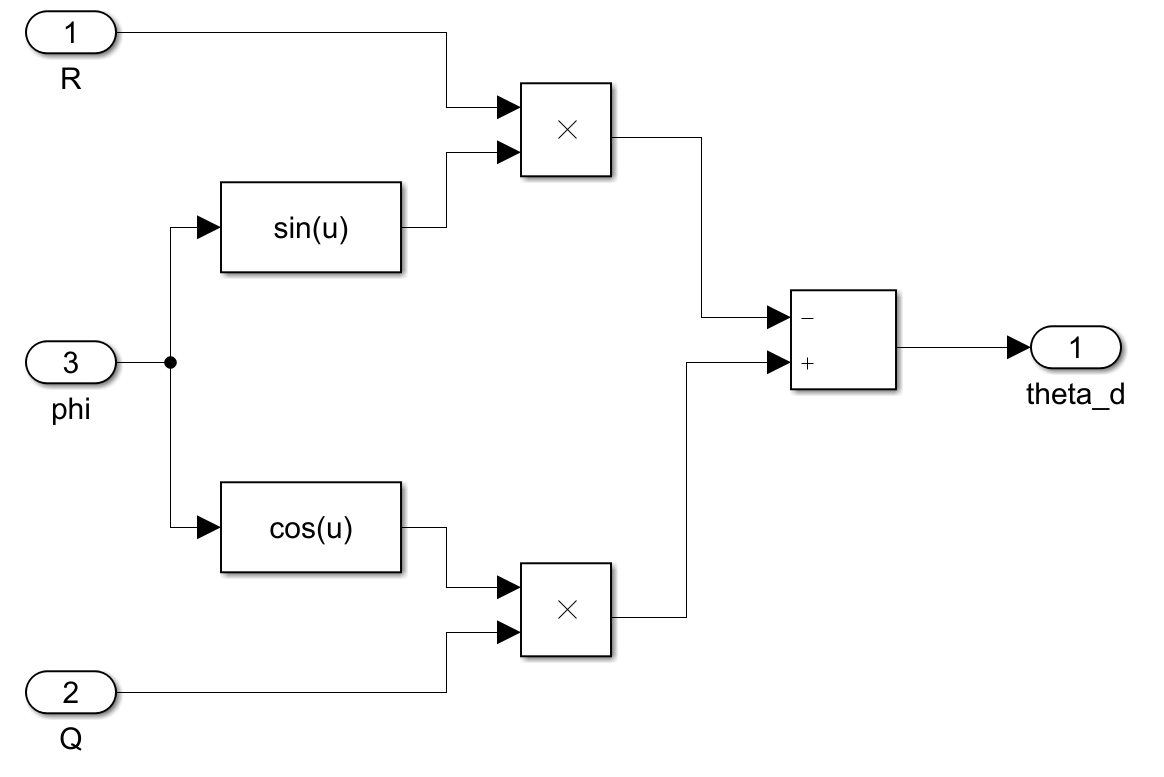
\includegraphics[width=\textwidth]{07_Thetad}
    \caption{$\dot{\Theta}$ Equation (6) Simulink Implementation}
    \label{fig:thetad}
\end{figure}

\begin{figure}[h]
    \centering
    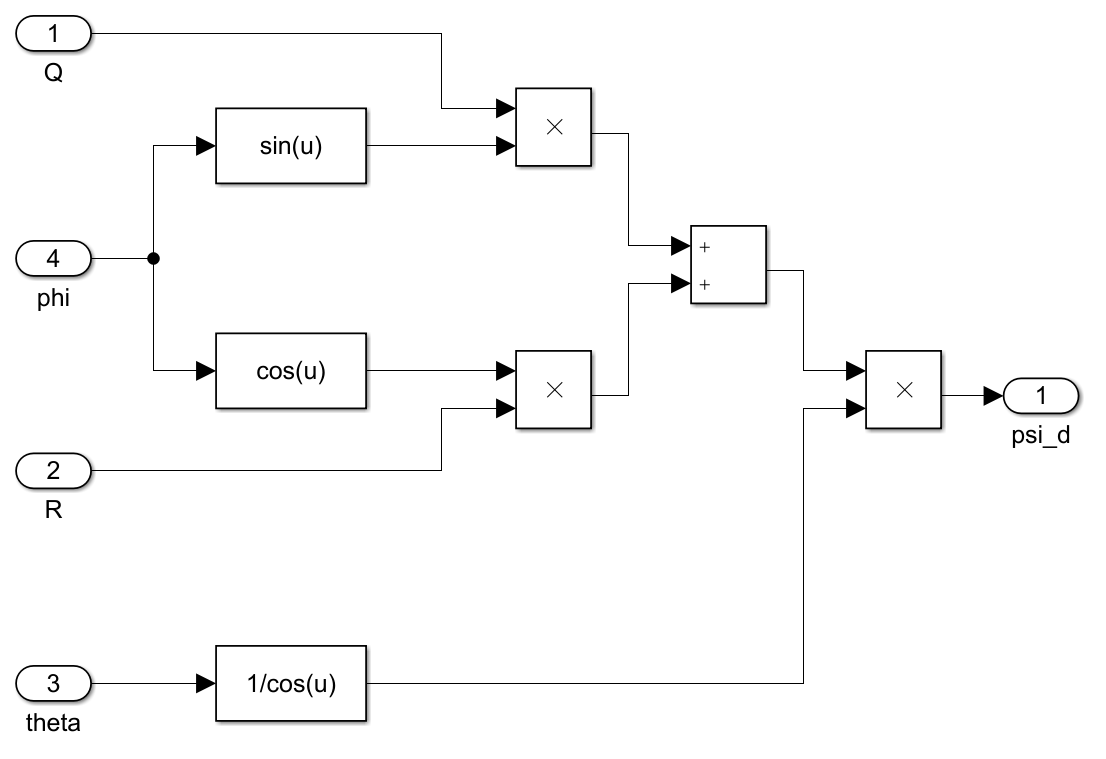
\includegraphics[width=\textwidth]{08_Psid}
    \caption{$\dot{\Psi}$ Equation (7) Simulink Implementation}
    \label{fig:psid}
\end{figure}

\begin{figure}[h]
    \centering
    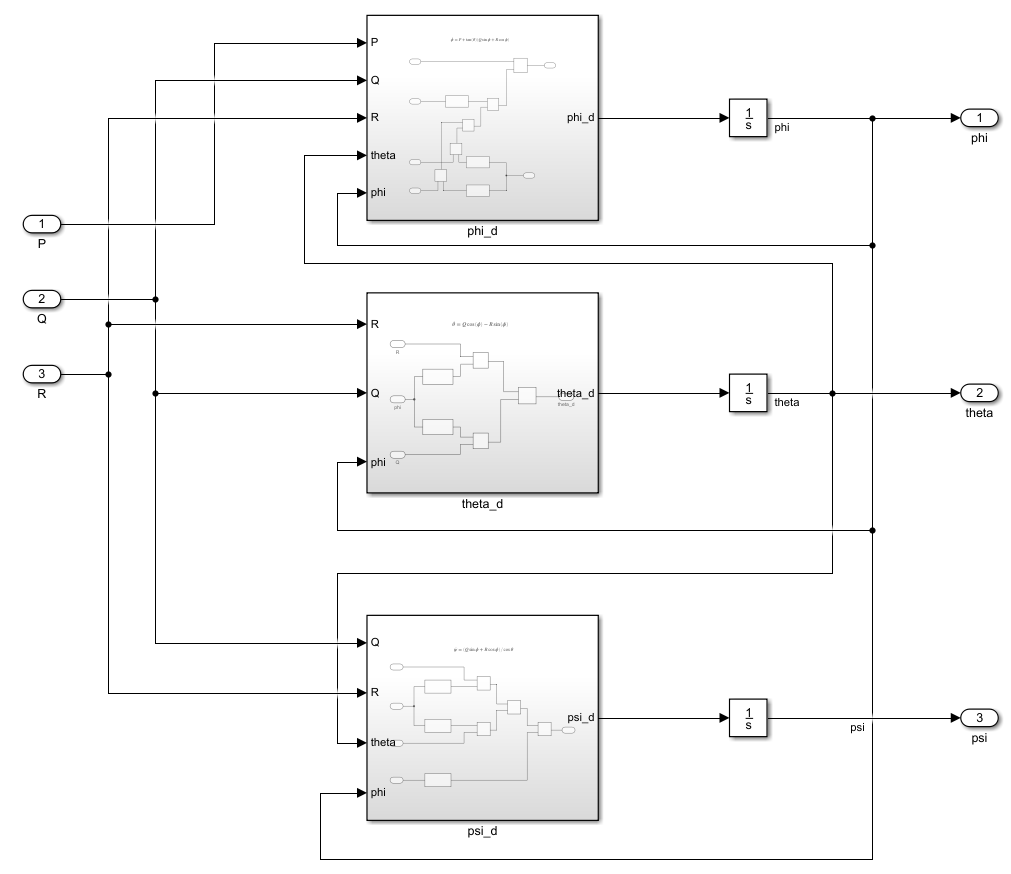
\includegraphics[width=\textwidth]{09_kinematic_equations}
    \caption{All 3 Kinematic Equation Subsystems Connected in Simulink}
    \label{fig:kine_eqns}
\end{figure}

% Moment Equations
\begin{figure}[h]
    \centering
    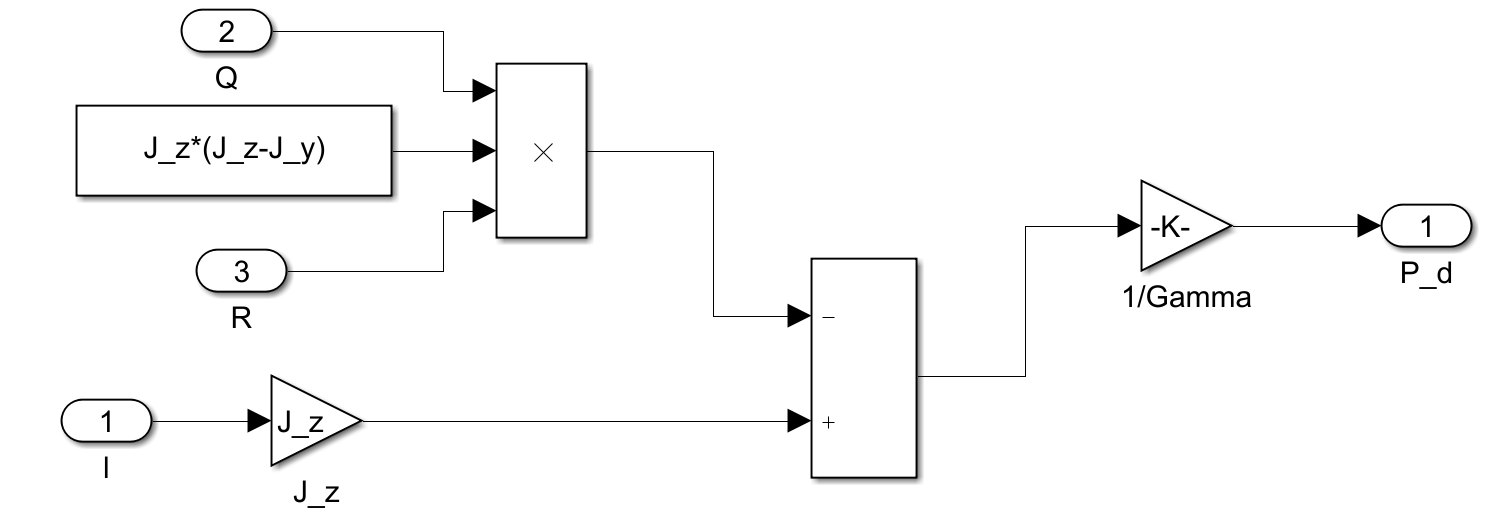
\includegraphics[width=\textwidth]{10_Pdot}
    \caption{$\dot{P}$ Equation (8) Simulink Implementation}
    \label{fig:Pd}
\end{figure}

\begin{figure}[h]
    \centering
    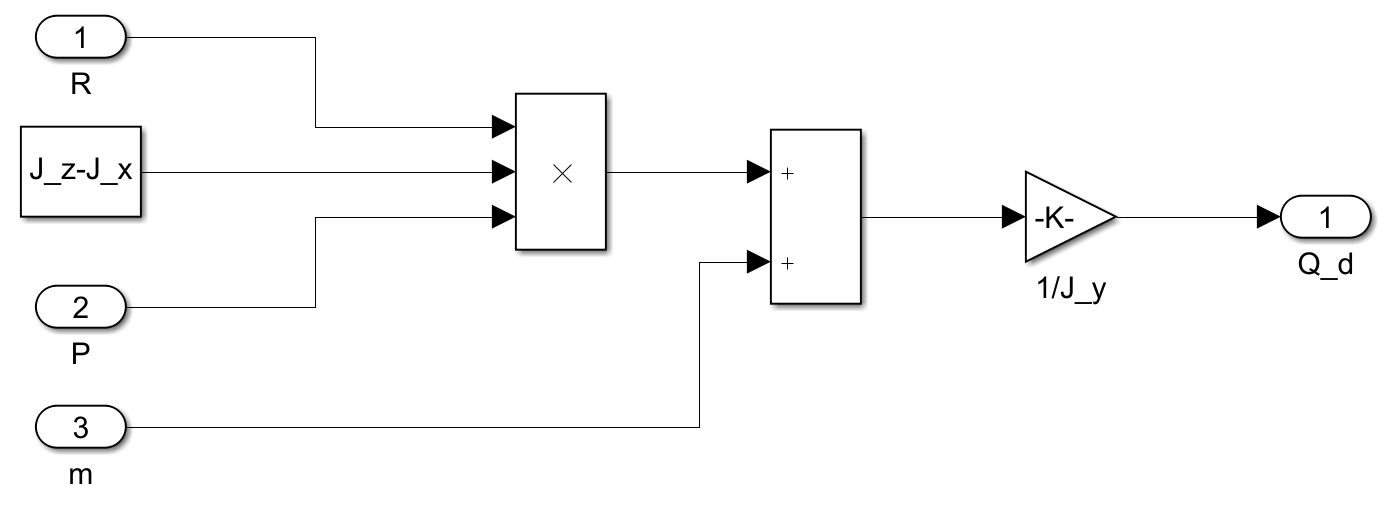
\includegraphics[width=\textwidth]{11_Qdot}
    \caption{$\dot{Q}$ Equation (9) Simulink Implementation}
    \label{fig:Qd}
\end{figure}

\begin{figure}[h]
    \centering
    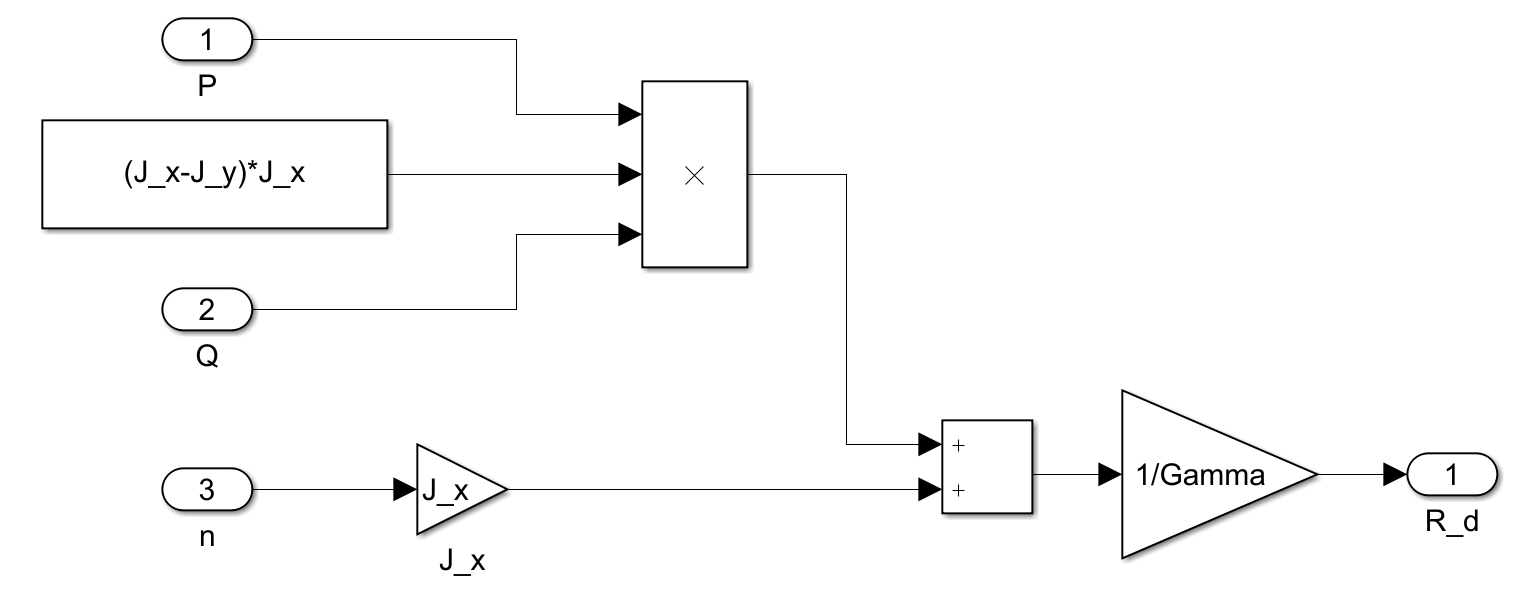
\includegraphics[width=\textwidth]{12_Rdot}
    \caption{$\dot{R}$ Equation (10) Simulink Implementation}
    \label{fig:Rd}
\end{figure}

\begin{figure}[h]
    \centering
    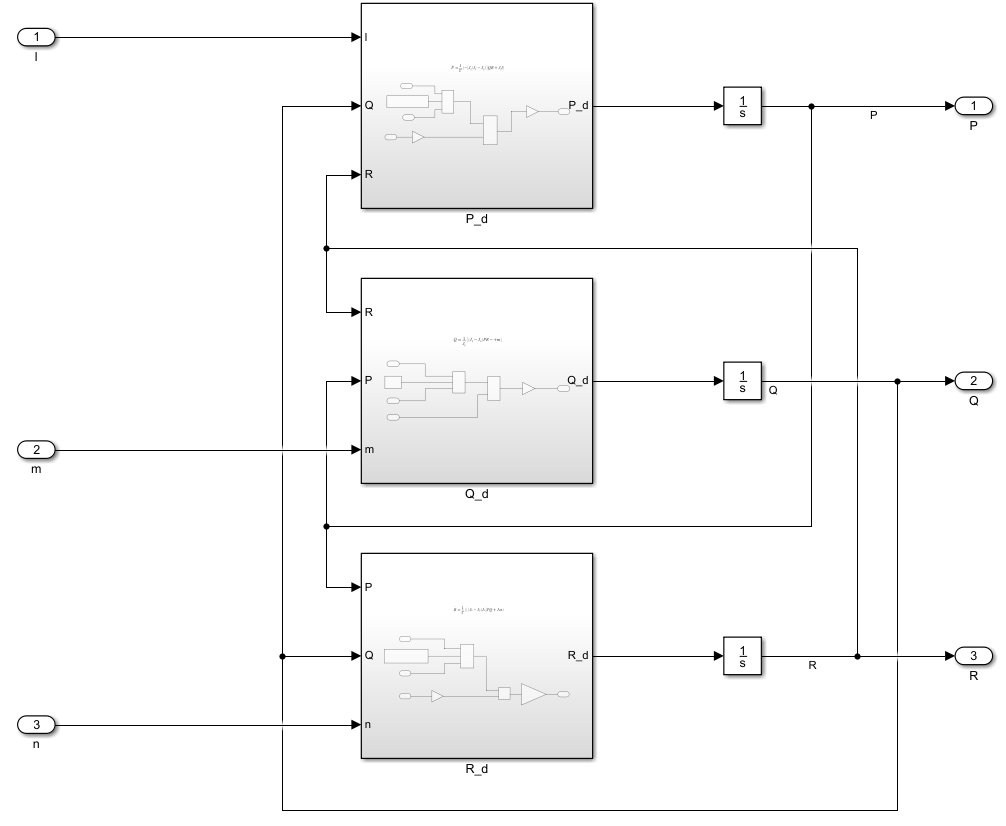
\includegraphics[width=\textwidth]{13_moment_equations}
    \caption{All 3 Moment Equation Subsystems Connected in Simulink}
    \label{fig:mom_eqns}
\end{figure}

% Navigation Equation
\begin{figure}[h]
    \centering
    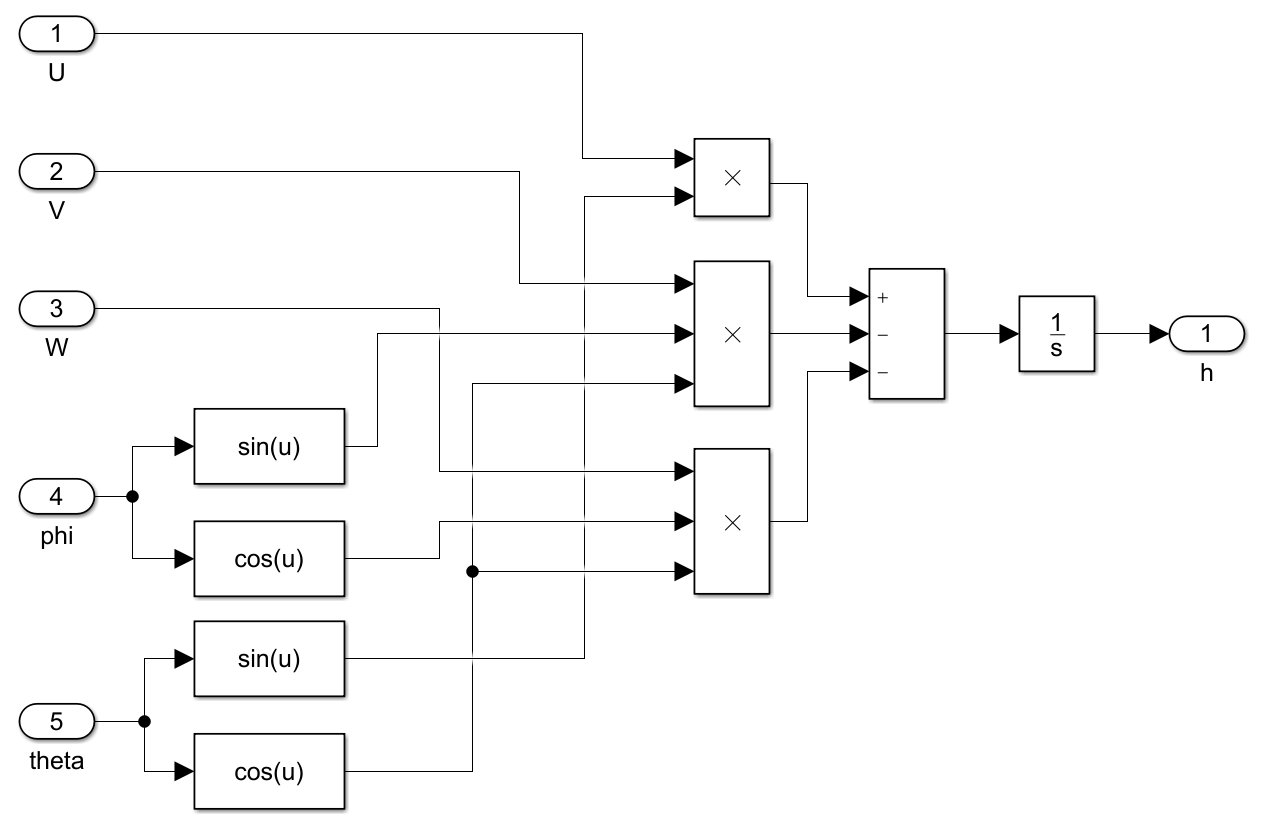
\includegraphics[width=\textwidth]{14_nav_eqn}
    \caption{$\dot{h}$ Equation (11) Simulink Implementation}
    \label{fig:nav_eqn}
\end{figure}

% 6-DOF Model
\begin{figure}[h]
    \centering
    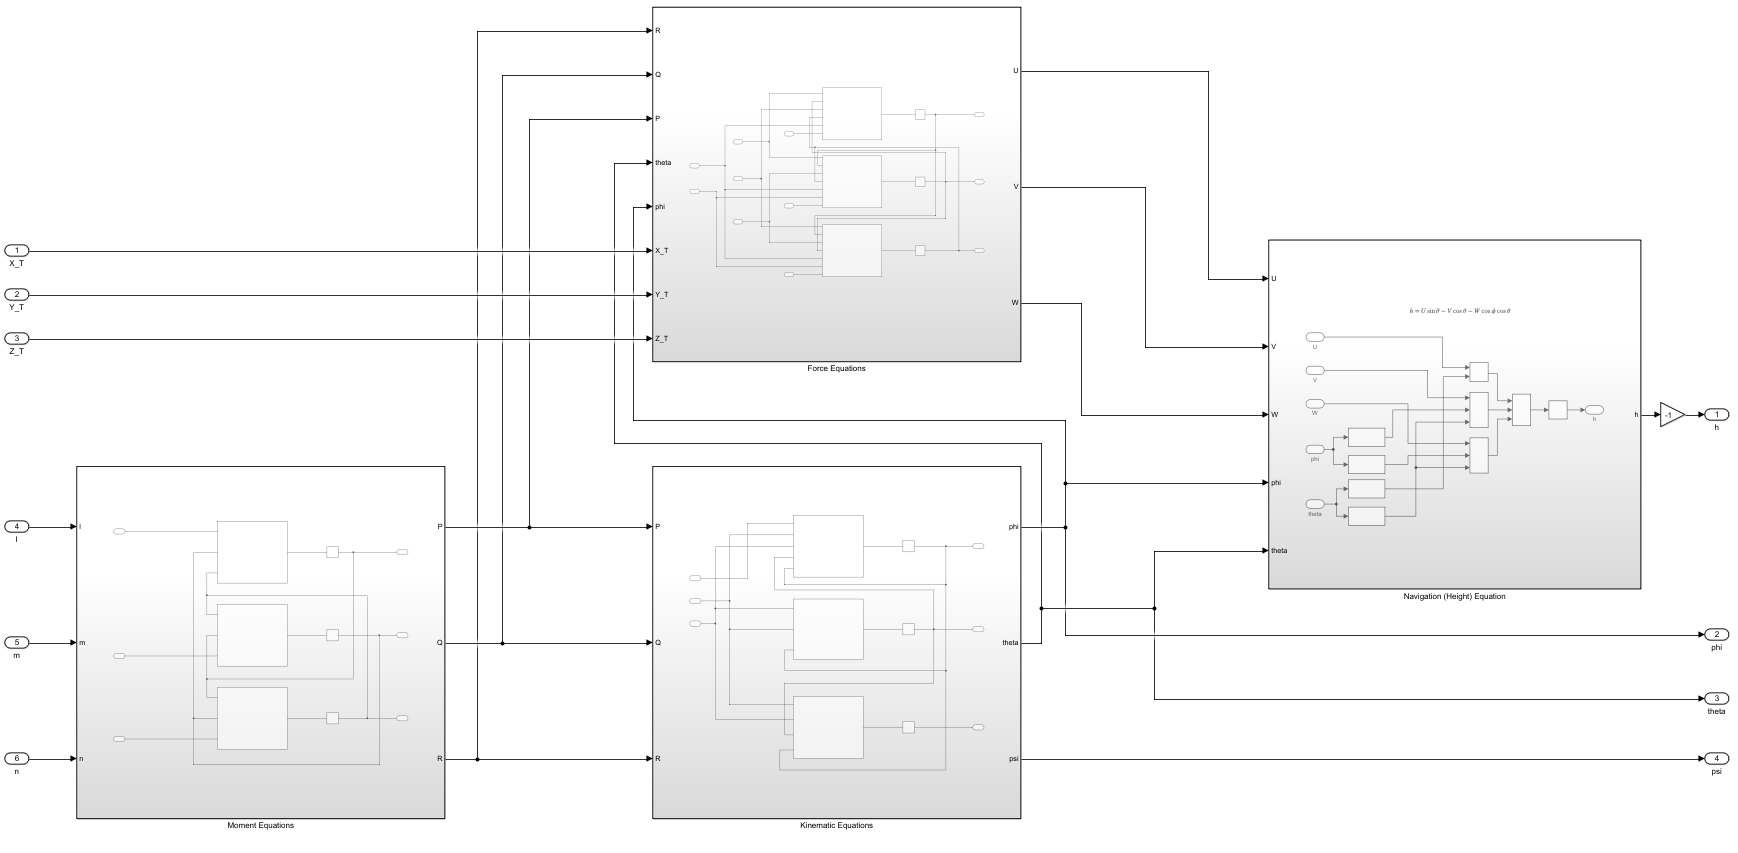
\includegraphics[width=1.25\textwidth, angle=90]{15_6dof}
    \caption{All 6-DOF Model Subsystems Connected in Simulink}
    \label{fig:6dof}
\end{figure}

% Physical Forces and Moments
\begin{figure}[h]
    \centering
    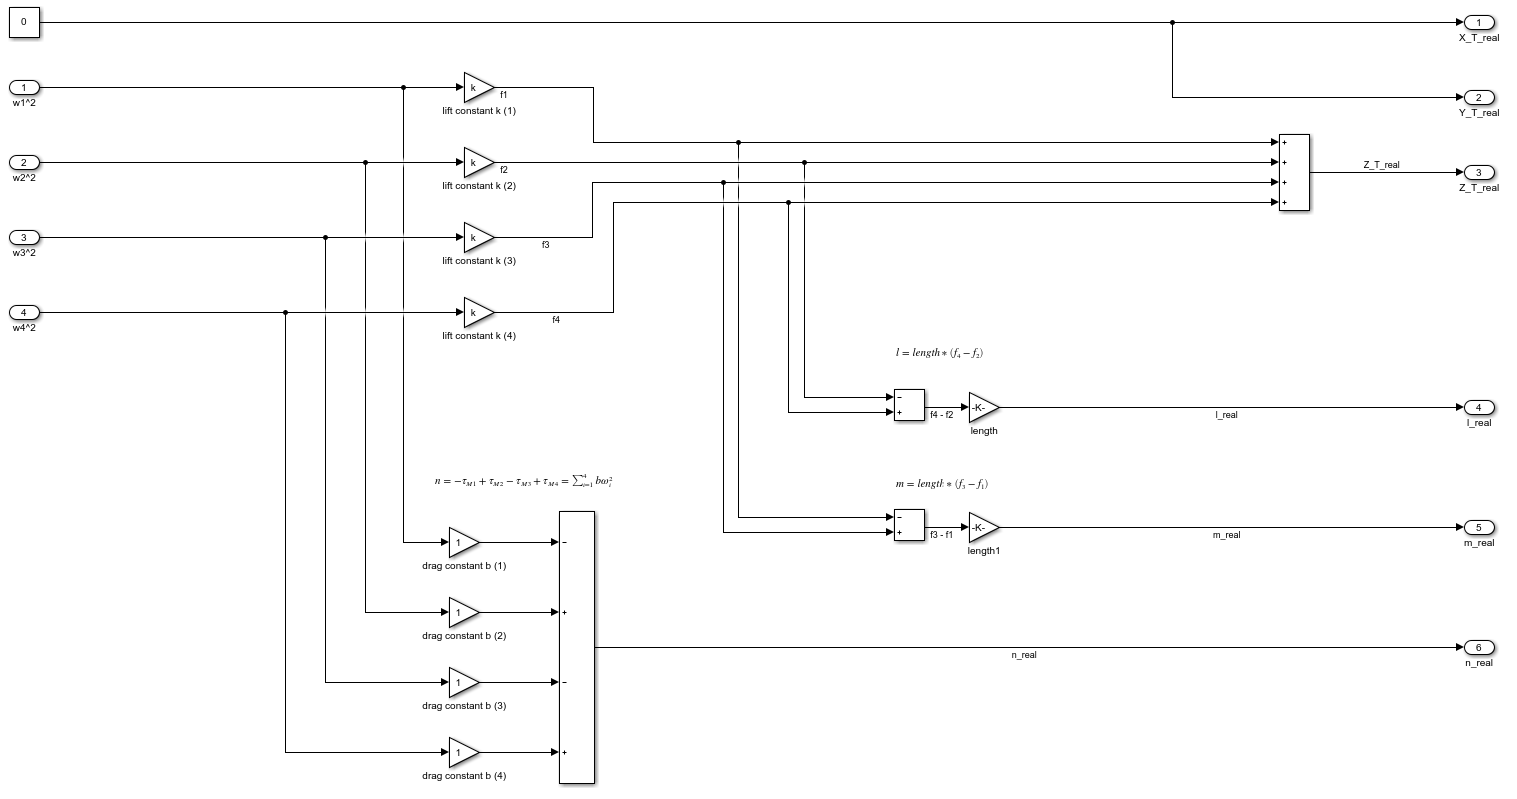
\includegraphics[width=\textwidth]{16_phys_force_mom}
    \caption{Physical Forces and Moments Equations in Simulink}
    \label{fig:phys_force_mom}
\end{figure}

% Control Allocation
\begin{figure}[h]
    \centering
    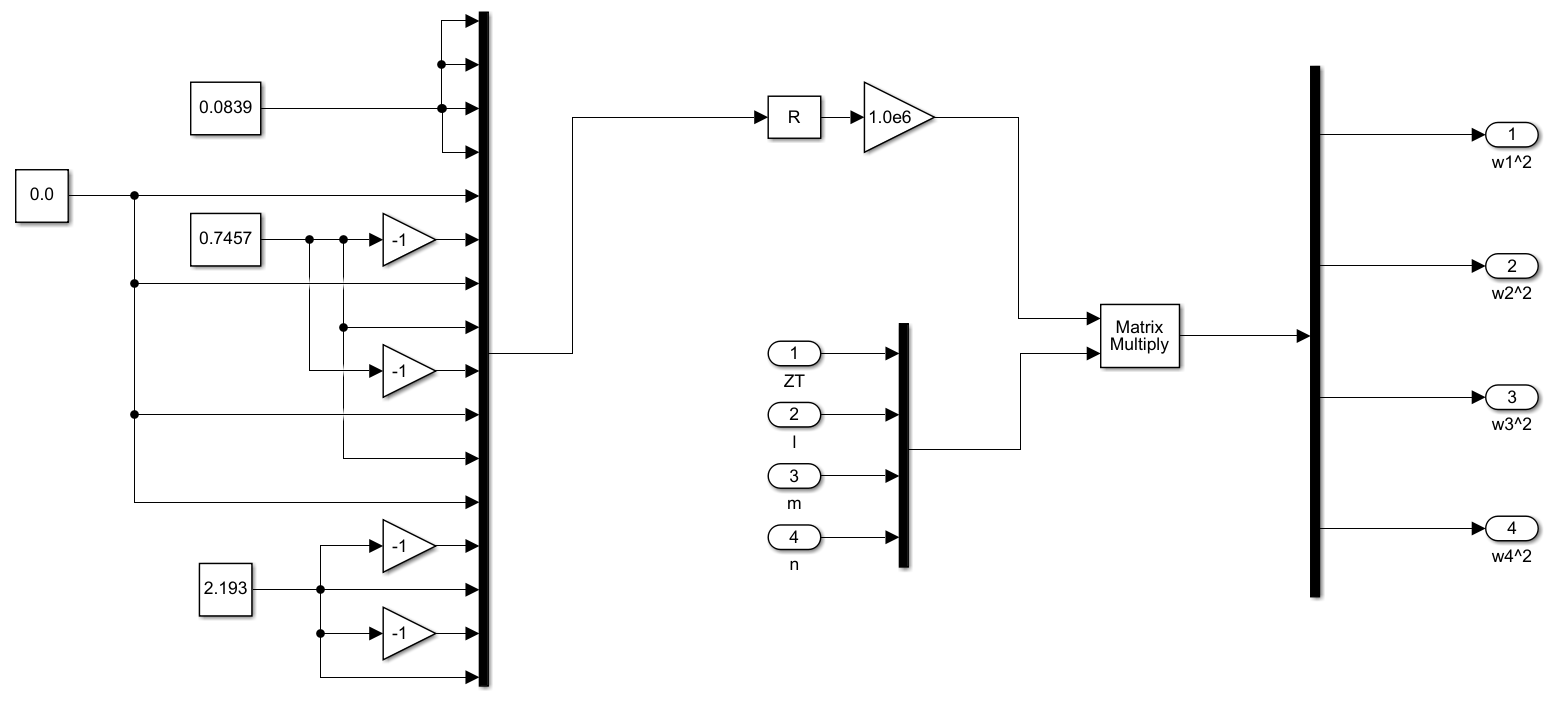
\includegraphics[width=\textwidth]{17_cont_alloc}
    \caption{Controller Allocation in Simulink}
    \label{fig:cont_alloc}
\end{figure}

% Controller
\begin{figure}[h]
    \centering
    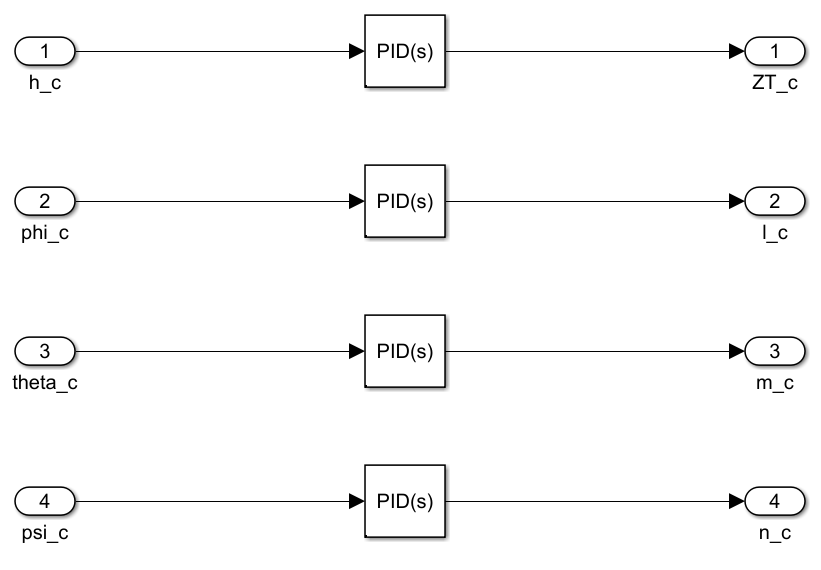
\includegraphics[width=\textwidth]{18_controller}
    \caption{PID Controllers in Simulink}
    \label{fig:cont}
\end{figure}

% Complete System
\begin{figure}[h]
    \centering
    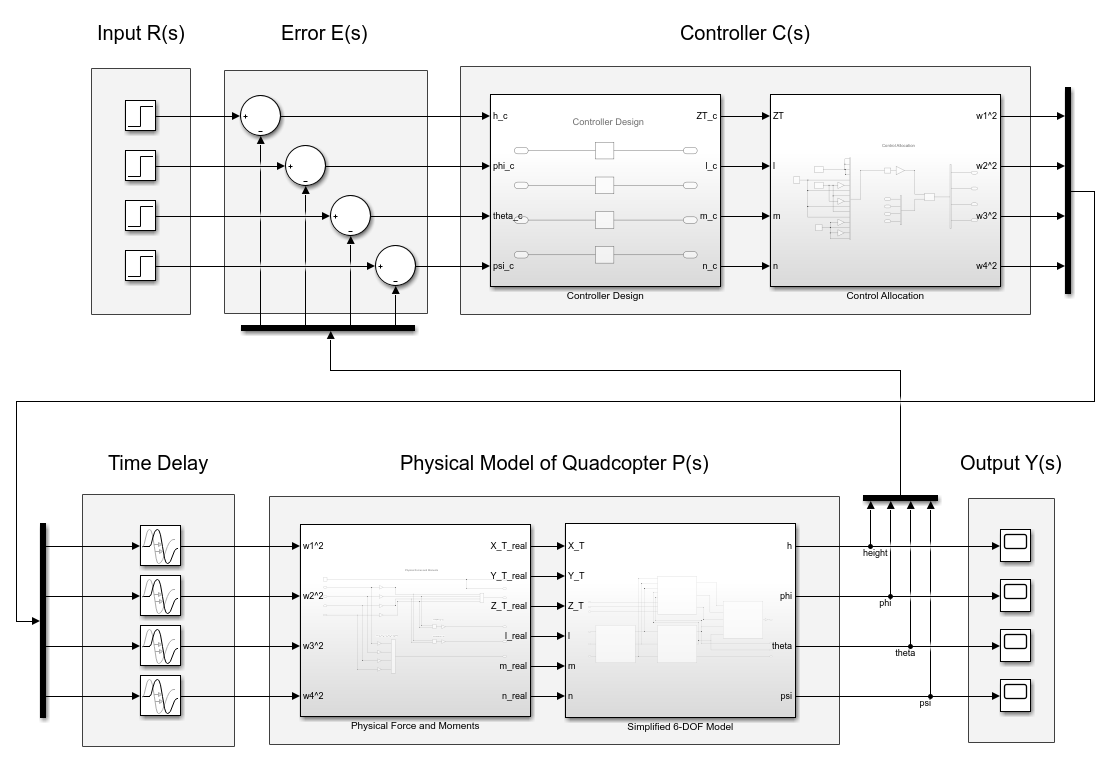
\includegraphics[width=\textwidth]{19_complete_system}
    \caption{The Entire System Represented in Simulink}
    \label{fig:}
\end{figure}

% Response Plots
\begin{figure}[h]
    \centering
    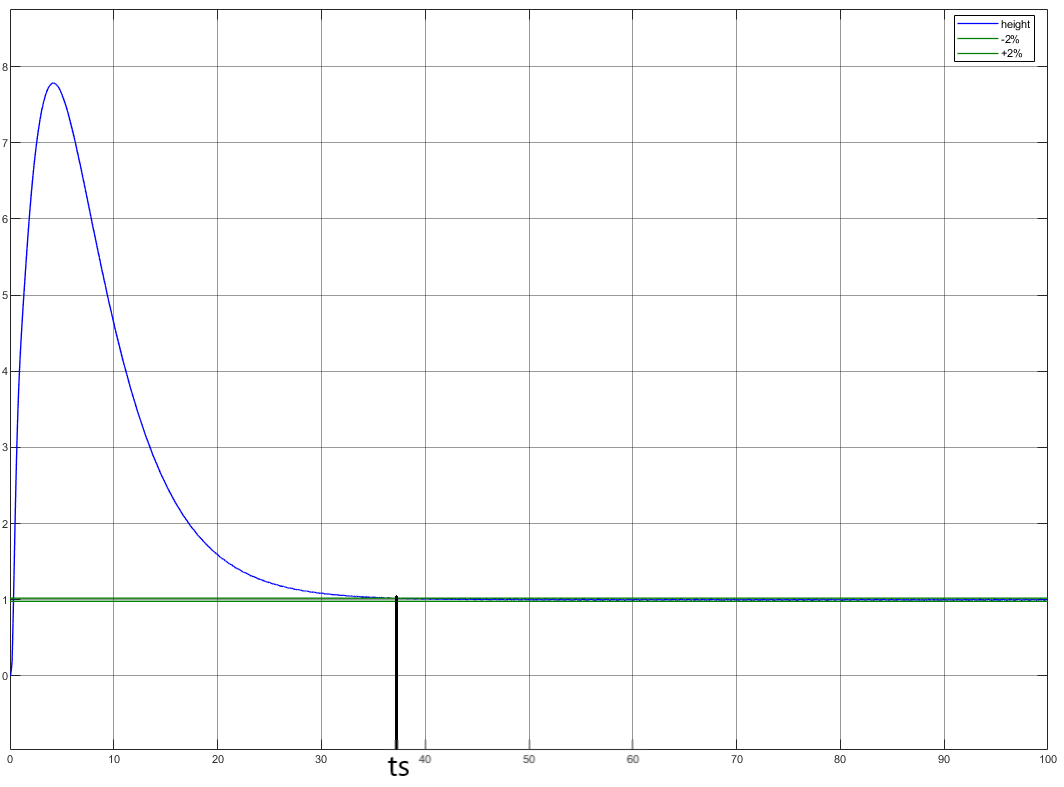
\includegraphics[width=\textwidth]{20_height}
    \caption{Height Response Plot}
    \label{fig:height}
\end{figure}

\begin{figure}[h]
    \centering
    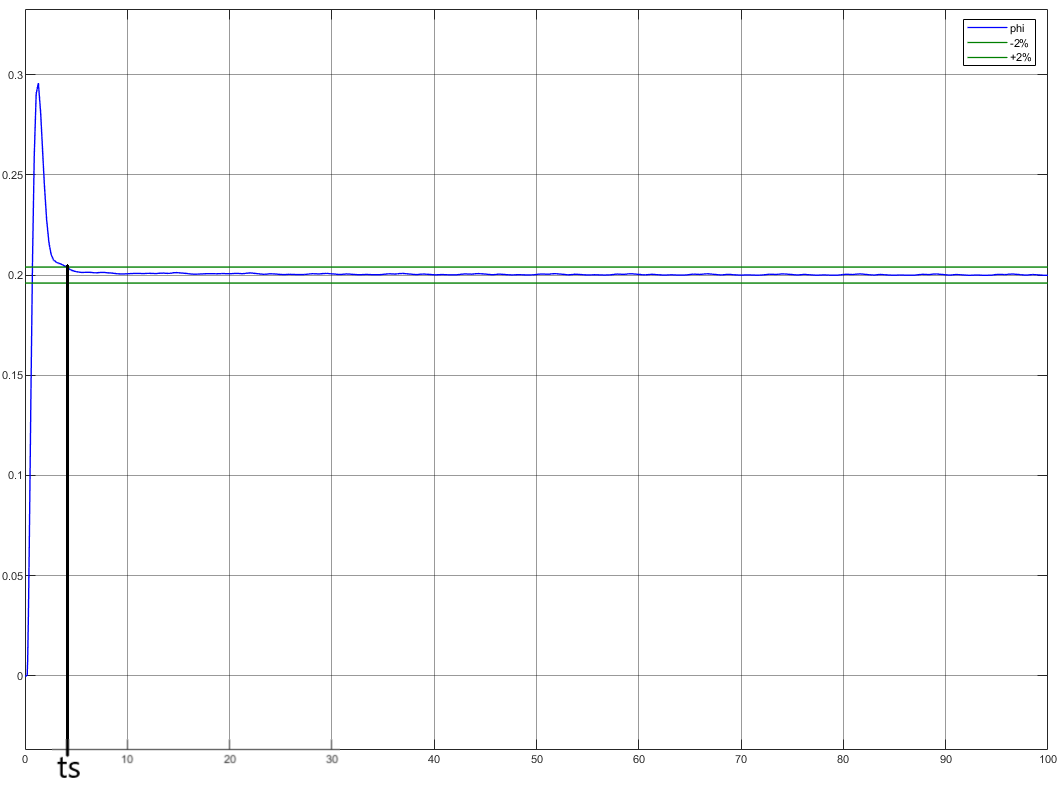
\includegraphics[width=\textwidth]{21_phi}
    \caption{Phi Response Plot}
    \label{fig:phi}
\end{figure}

\begin{figure}[h]
    \centering
    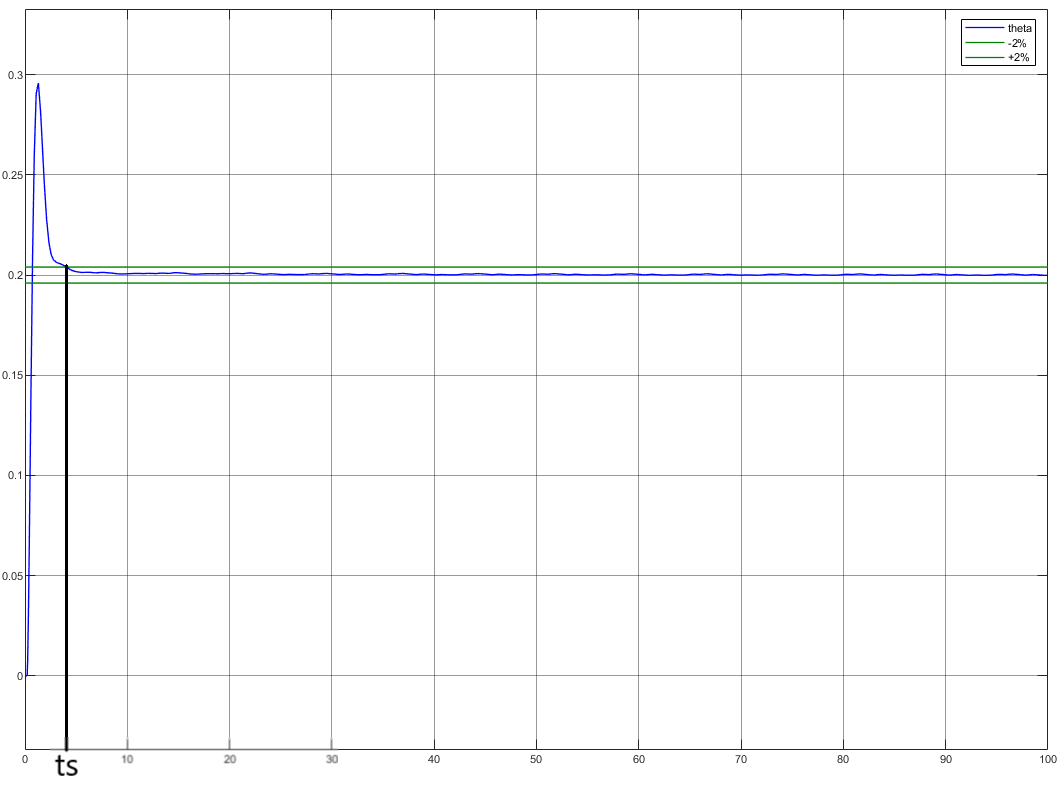
\includegraphics[width=\textwidth]{22_theta}
    \caption{Theta Response Plot}
    \label{fig:theta}
\end{figure}

\begin{figure}[h]
    \centering
    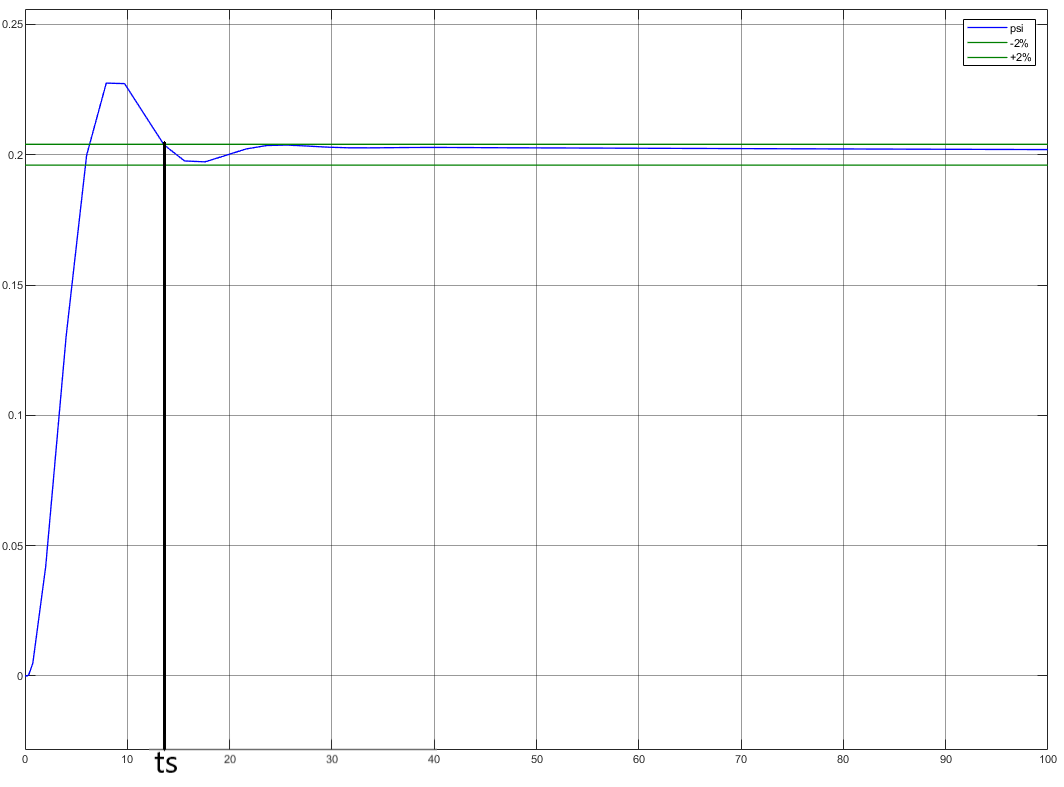
\includegraphics[width=\textwidth]{23_psi}
    \caption{Psi Response Plot}
    \label{fig:psi}
\end{figure}